\begin{figure}[t]
    \centering
    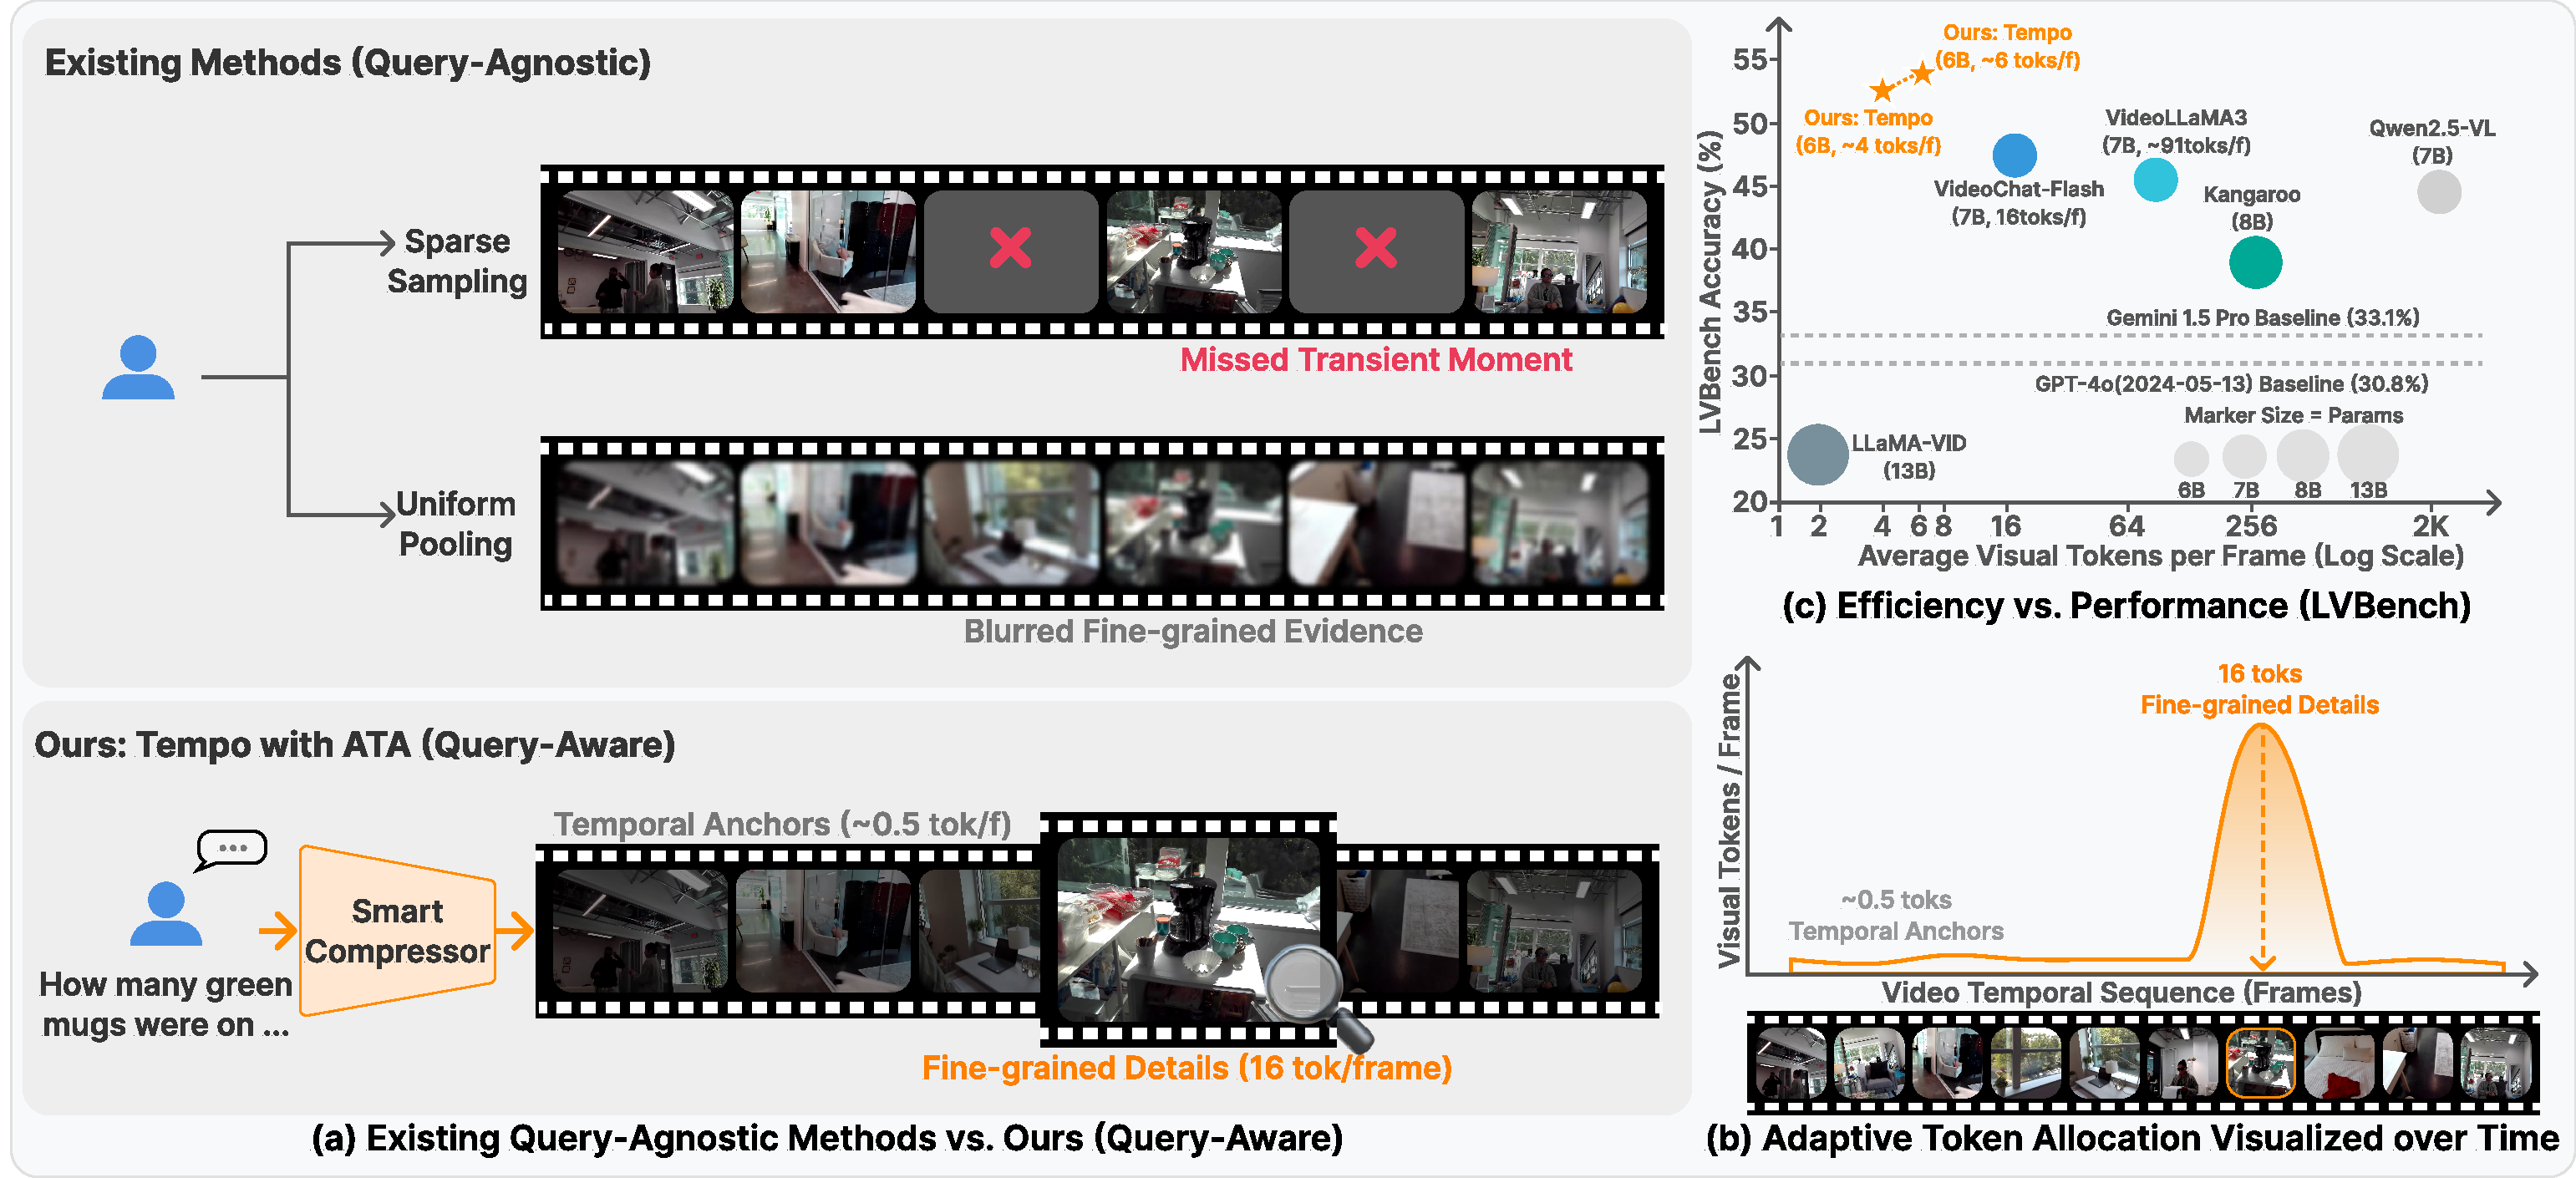
\includegraphics[width=\textwidth]{fig/teaser.pdf}
    \caption{
    \textbf{Tempo achieves SOTA long video understanding via query-aware Adaptive Token Allocation (ATA).}
    \textbf{(a) Motivation:} Query-agnostic methods either miss transient moments (sparse sampling) or blur details (uniform pooling). Tempo instead utilizes a small vision-language model as a \emph{smart compressor} for query-aware cross-modal distillation.
    \textbf{(b) Mechanism:} ATA dynamically allocates high bandwidth (16 tokens/frame) to relevant segment for fine-grained details, while compressing redundant contexts into minimal temporal anchors ($\sim$0.5 tokens/frame) to maintain causality.
    \textbf{(c) Result:} Leading performance on LVBench. Tempo-6B achieves superior accuracy at extreme compression rates (\ie, 4 or 6 tokens/frame), outperforming open-source models and proprietary baselines with a fraction of the context budget.
    }
    % \vspace{-1em}
    \label{fig:teaser}
\end{figure}